% Generated by scripts/make_census_figures.py -- do not edit by hand.
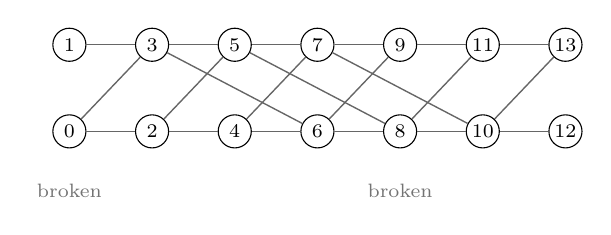
\begin{tikzpicture}[
  x=1cm, y=1cm,
  el/.style={circle, draw, minimum size=4.2mm, inner sep=1pt,
             font=\scriptsize},
  rail/.style={draw=black!60, line width=0.5pt},
  rung/.style={draw=black!60, line width=0.5pt},
]
  \node[el] (l0) at (0.00,0.00) {0};
  \node[el] (l1) at (0.00,1.10) {1};
  \node[el] (l2) at (1.05,0.00) {2};
  \node[el] (l3) at (1.05,1.10) {3};
  \node[el] (l4) at (2.10,0.00) {4};
  \node[el] (l5) at (2.10,1.10) {5};
  \node[el] (l6) at (3.15,0.00) {6};
  \node[el] (l7) at (3.15,1.10) {7};
  \node[el] (l8) at (4.20,0.00) {8};
  \node[el] (l9) at (4.20,1.10) {9};
  \node[el] (l10) at (5.25,0.00) {10};
  \node[el] (l11) at (5.25,1.10) {11};
  \node[el] (l12) at (6.30,0.00) {12};
  \node[el] (l13) at (6.30,1.10) {13};
  \draw[rail] (l0) -- (l2);
  \draw[rung] (l0) -- (l3);
  \draw[rail] (l1) -- (l3);
  \draw[rail] (l2) -- (l4);
  \draw[rung] (l2) -- (l5);
  \draw[rail] (l3) -- (l5);
  \draw[rung] (l3) -- (l6);
  \draw[rail] (l4) -- (l6);
  \draw[rung] (l4) -- (l7);
  \draw[rail] (l5) -- (l7);
  \draw[rung] (l5) -- (l8);
  \draw[rail] (l6) -- (l8);
  \draw[rung] (l6) -- (l9);
  \draw[rail] (l7) -- (l9);
  \draw[rung] (l7) -- (l10);
  \draw[rail] (l8) -- (l10);
  \draw[rung] (l8) -- (l11);
  \draw[rail] (l9) -- (l11);
  \draw[rail] (l10) -- (l12);
  \draw[rung] (l10) -- (l13);
  \draw[rail] (l11) -- (l13);
  \node[font=\scriptsize, black!55] at (0.00,-0.75) {broken};
  \node[font=\scriptsize, black!55] at (4.20,-0.75) {broken};
\end{tikzpicture}
